\section{Game}
In \secref{processweek2} i we mentioned that main functionality of the game interface is drag and drop. During the early stages of project we created a simple prototype of the game and its interface. We had different views on whether the game should be a top-down perspective or side-scrolling. We decided on the side-scrolling perspective since it would be easier to perform drag and drop actions.
\subsection{Game Idea/Description}
%Skriv hvordan spillet fungere
In \secref{processweek2} it is explained how Tove's version of the exercise work. We intent keep the same principles of Tove's exercise.
\subsubsection*{Game objects}
\begin{description}
\item[Pictogram] Is a object which contains a picture and is draggable.
\item[Train Station] Is a station where the train stops, and allows the child to drag and drop pictograms onto the station. Each station has a picture indicating the category of the station. The category of the station describes the pictograms that should be dropped onto the station.  

\item[Flute] Is a button that the child can press if they think that the correct pictograms have been dropped onto the station. If however the child have made a mistake and dropped a pictogram not belonging to the station's category, then the train would not start.

\item[Train and wagons] Is a vehicle that drives to each station, carrying pictograms in its wagons.

\item[Landscape sequence] Is a sequence of hills, trees, cow, and skies. The landscape sequence is placed between each stations, and creates the illusion that the train is driving to the next station.
\item[Train depot] When the train is driving from the last Train station, the train will drive into the a train depot to indicate the the game is over.
\end{description}

\subsubsection*{Game Flow}
\todo{this section describes the flow of the game}
Our game starts by the child must drag the pictograms off the start Train station and drop them onto the train, the start station is special since it does not have a category. The start station is to help the child understand how to move pictures with drag and drop. When the child have moved all the pictures onto the train, it is allowed to drive through a landscape sequence, until it reaches the first train station.
The Train station has a category, which could be a picture of animals. It is now up to the child to drag all the animals off the train onto the station, so the train can continue. If all the right pictograms is on the station, the train will drive onto the next station or train depot.
When the train has reached the train depot, it the child is presented with a button saying "God job!", indicating that the game is over.

\subsection{Game Prototype}
\todo{explain the prototype, and the what Tove liked, and would like add or change}
%vis billedet af prototypen, beskriv hvad Tove godt kunne lide, og hvad der kunne ændres, samt tilføjelser. (fløjten, ingen musik, no fancy colors on objects)
\begin{figure}[H]
\centering
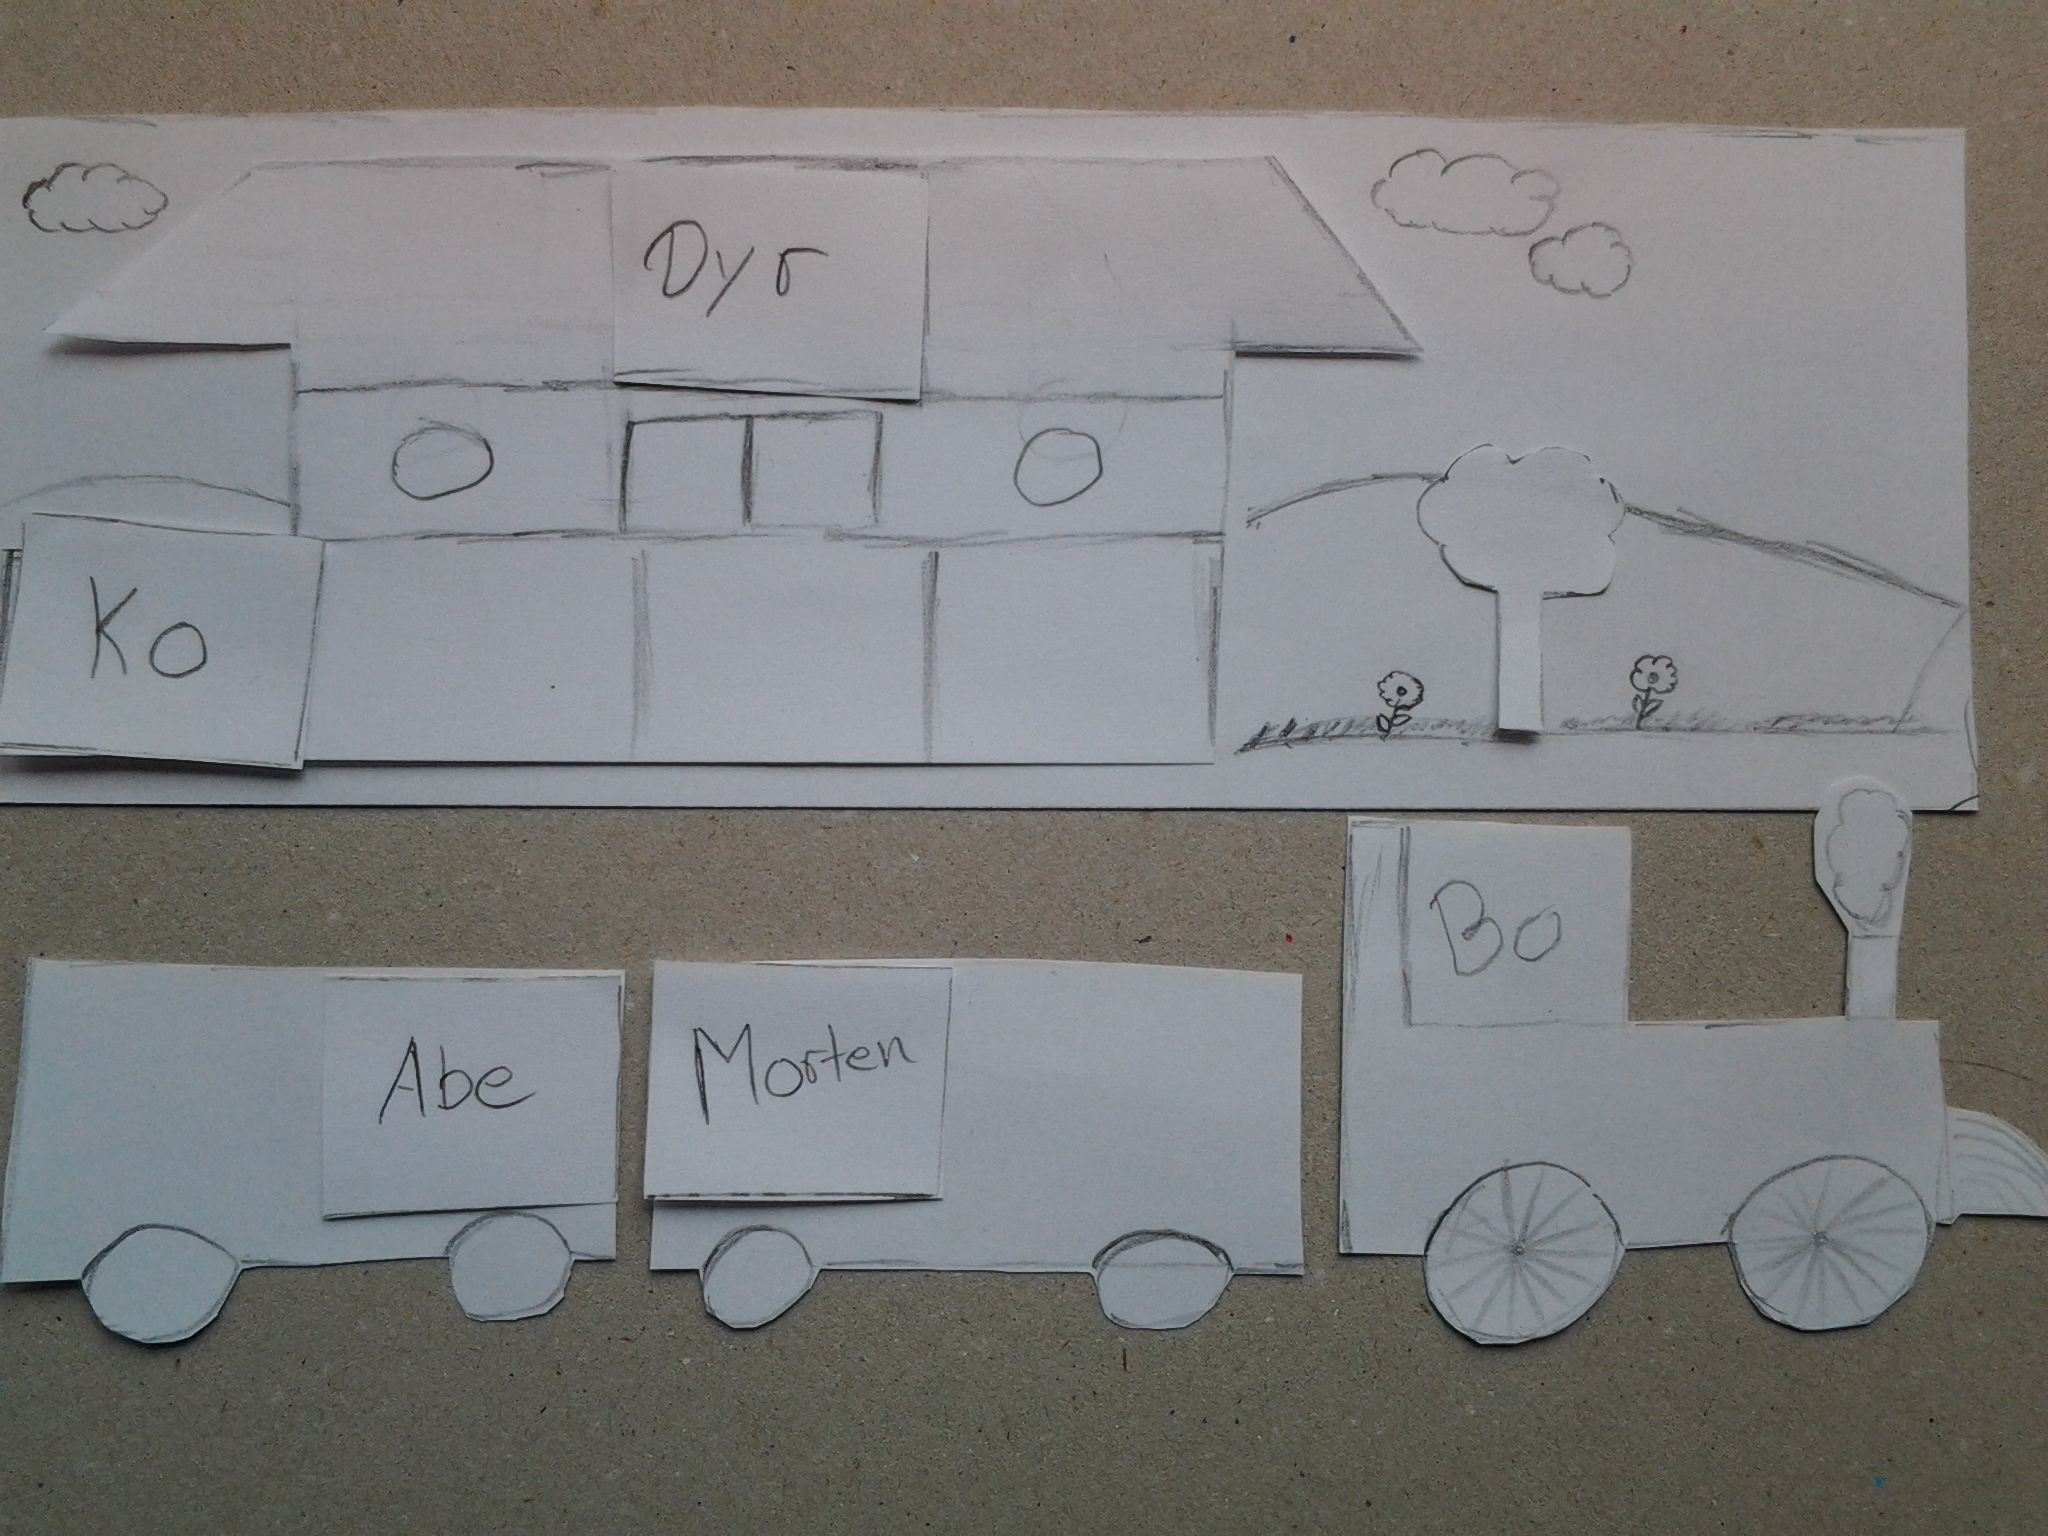
\includegraphics[width=0.9\linewidth]{img/screenshots/prototype1.jpg}%0.1 margin
\caption{The paper prototype}
\label{fig:paperprototype}
\end{figure}
\autoref{fig:paperprototype} shows the paper prototype we showed Tove at our first meeting. We explained the our game idea. She liked the idea and the interface, although she wished to see a button that would check if the correct pictograms was off the train, and start the train. She also mentioned that the game should not contain many different colors and sounds, since this would cause visual and audible noise for the child.


\subsection{Game Interface}
\todo{Final result, with picture}
\begin{figure}[H]
\centering
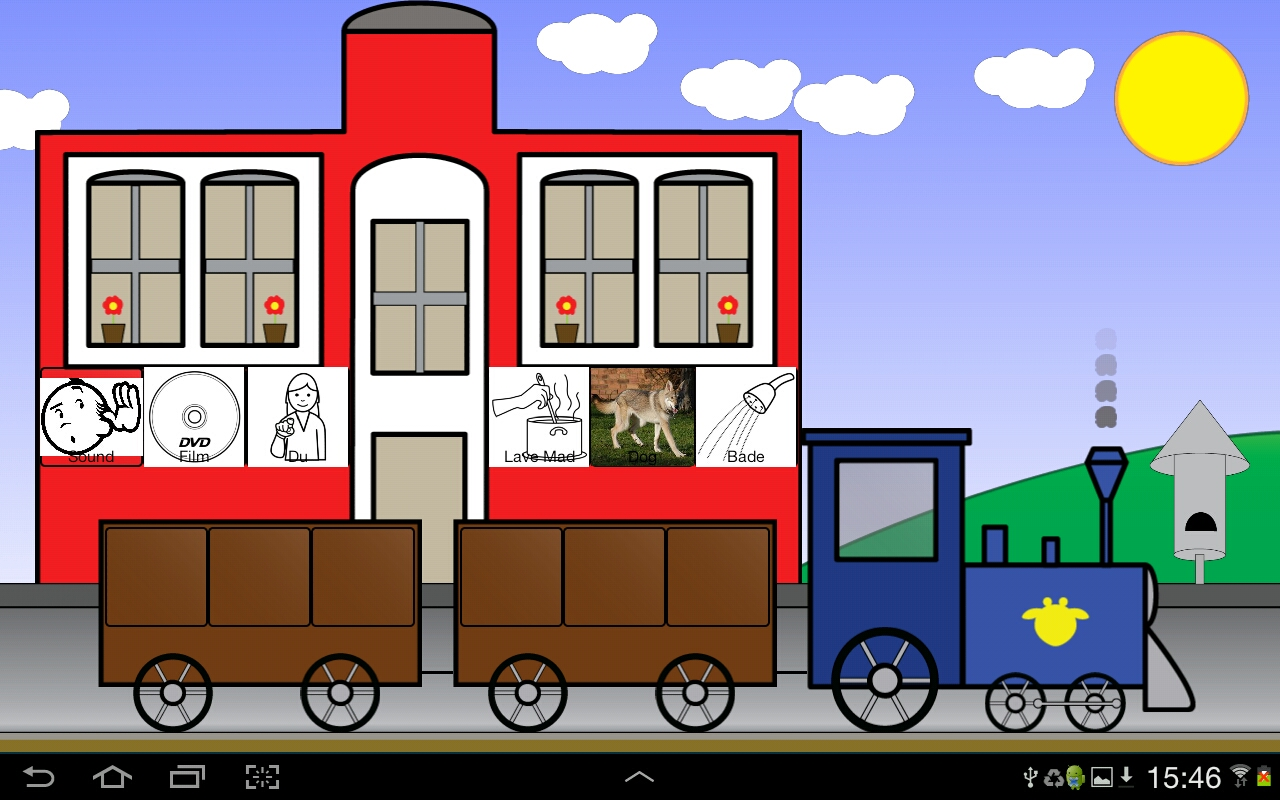
\includegraphics[width=0.9\linewidth]{img/screenshots/gamedesign1.jpg}%0.1 margin
\caption{The final result}
\label{fig:finalresult}
\end{figure}
During the project we sent screen shots of the game interface to Tove, to confirm that we were on the right track. For the most part she had not much to add, only small graphical adjustments to stations. In order to mimic Tove's version of the exercise we had to make the game customizable.
%hvis det endelig resultat, samt de ting som ikke noget at blive tilføjet.(Traindriver, click and autosnap, lyd på pictogrammer)
